\documentclass{article}
\usepackage[x11names, svgnames, rgb]{xcolor}
\usepackage[utf8]{inputenc}
\usepackage{tikz}
\usetikzlibrary{snakes,arrows,shapes}
\usepackage{amsmath}
%
%

%

%

\begin{document}
\pagestyle{empty}
%
%
%

\enlargethispage{100cm}
% Start of code
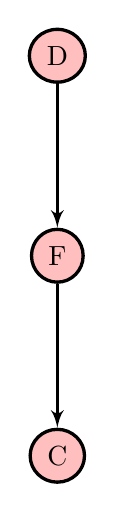
\begin{tikzpicture}[>=latex',line join=bevel, line width=1.2pt]
%%
\node (D) at (27.0bp,162.0bp) [draw,fill=pink,ellipse] {D};
  \node (F) at (27.0bp,90.0bp) [draw,fill=pink,ellipse] {F};
  \node (C) at (27.0bp,18.0bp) [draw,fill=pink,ellipse] {C};
  \draw [->] (D) ..controls (27.0bp,136.13bp) and (27.0bp,126.97bp)  .. (F);
  \draw [->] (F) ..controls (27.0bp,64.131bp) and (27.0bp,54.974bp)  .. (C);
%
\end{tikzpicture}
% End of code

%
\end{document}
%



